\documentclass[aspectratio=169]{beamer}
\usetheme[language=ngerman,
titlepagelogo=logopolito,
bullet=circle,
pageofpages=of,
titleline=true,
color=blue
]{TorinoTh}

%\usepackage[ngerman]{babel}
%\usepackage[utf8]{inputenc}
\usepackage{tabularx}
\usepackage{booktabs}
\usepackage{multicol}
\usepackage{ulem}
\usepackage{makecell}
\usepackage{upgreek}
\usepackage{movie15}
%\usepackage{isodate}

\addto{\captionsngerman}{%
  \renewcommand*{\contentsname}{Contents}
  \renewcommand*{\listfigurename}{Figures}
  \renewcommand*{\listtablename}{Tables}
  \renewcommand*{\figurename}{Fig.}	
  \renewcommand*{\tablename}{Tab.}
}
\newcommand*\mean[1]{\bar{#1}}
\newcommand{\tabitem}{~~\llap{\textbullet}~~}
\newcommand\widebar[1]{\mathop{\overline{#1}}}

\usepackage{color}
\usepackage{graphicx}
\usepackage{fancybox}

\usepackage{beamerthemesplit}
\usetheme[compress]{Heidelberg}
\definecolor{unirot}{rgb}{0.4,0.4,0.3} % babyblue 0,0.58,1
\usecolortheme[named=unirot]{structure}
%\setbeamercolor{alerted text}{fg=red}
\newcommand*\hilite[1]{\textcolor{red}{#1}}
%\def\hilite<#1>{%
  %\temporal<#1>{\color{black}}{\color{unirot}}%
               %{\color{gray}}}


\title[Light Transport Techniques for Tensor Field Visualization]{Light Transport Techniques for Tensor Field Visualization}
\subtitle{Master's Thesis Presentation}
\vspace*{2pt}
\author[Sebastian Bek]{Sebastian Bek\vspace*{7pt}}
\date{July 24th 2019}
\institute[Uni HD]{
Heidelberg University\\
Visual Computing Group (VCG)\\
Supervisors: Prof. Filip Sadlo, Dr. Susanne Krömker\\
}

%\color{unirot}{sebibek@gmail.com}
%\newsubfloat{figure}
\newcommand{\source}[1]{\vspace{-3pt} \caption*{ Source: {#1}} }
\setlength{\belowcaptionskip}{-10pt}
\setlength{\intextsep}{-30pt}

\begin{document}

%\frame[plain]{\titlepage}

\frame{
\frametitle{{Light Transport Gradient - Heart dataset}}
\begin{figure}[!t]
\centering
  \begin{minipage}{0.3\textwidth}
   \centering
  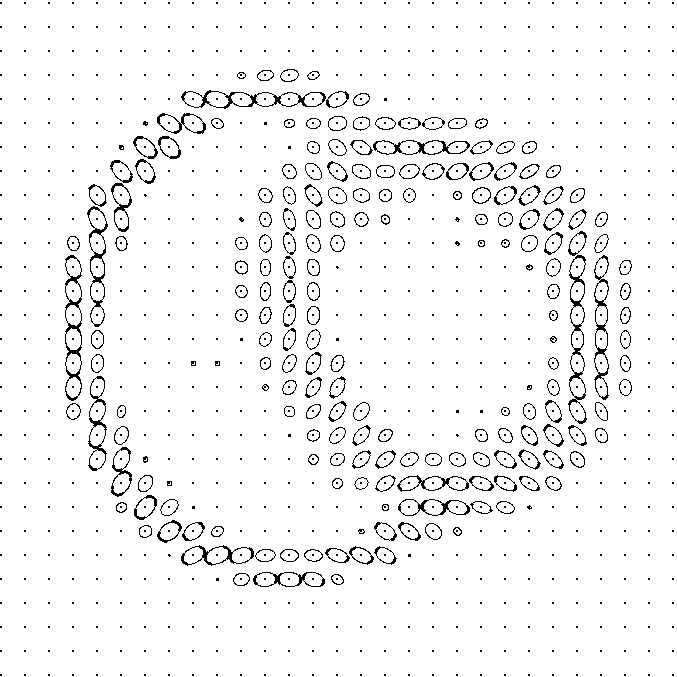
\includegraphics[width=0.7\textwidth]{heartDwnsmpl.png}
	a)
    \label{a)}
  \end{minipage}
  \begin{minipage}{0.3\textwidth}
   \centering
    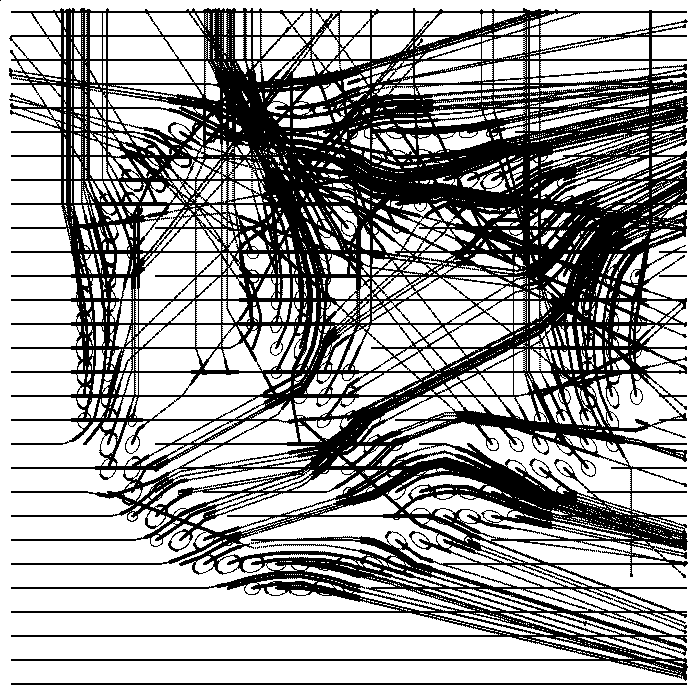
\includegraphics[width=0.7\textwidth]{heartDwnsmpl-TFL.PNG}
	b)
    \label{b)}
  \end{minipage}
  \begin{minipage}{0.3\textwidth}
   \centering
    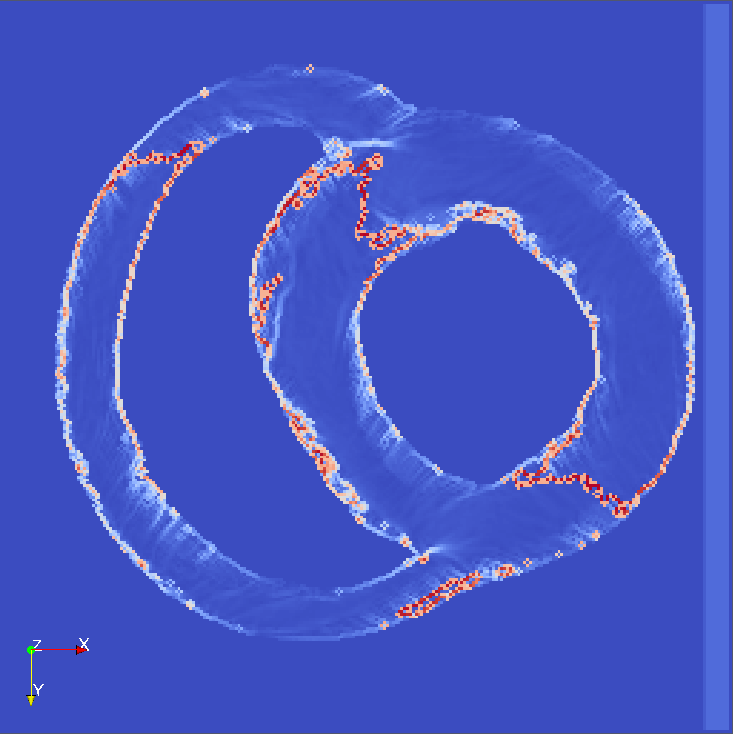
\includegraphics[width=0.7\textwidth]{heart_ftle_org.PNG}
	c)
    \label{b)}
  \end{minipage}
\caption{Heart test field: a) glyphs, b) TFLs, c) FTLE: H.'s approach}
\label{heart-ftle-comp}
\end{figure}


\begin{itemize}
	\item No noise present in the Heart dataset $\Rightarrow$ TFLs reveal correlated trajectories
	\item FTLE response on structure obtained in the style of Hlawatsch et al.
\end{itemize}
} % END OF FRAME

\frame{
\frametitle{{Heart dataset - Evaluation}}
\begin{figure}[!t]
\centering
  \begin{minipage}{0.3\textwidth}
  \centering
  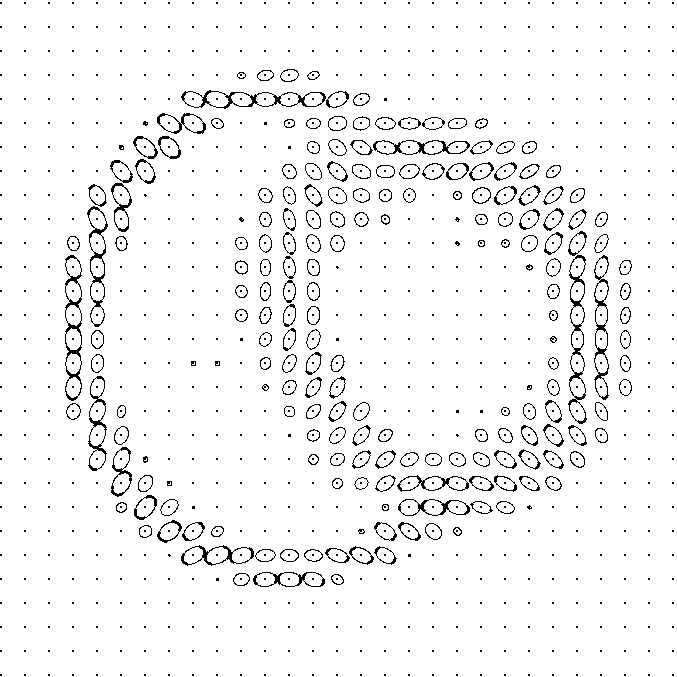
\includegraphics[height=0.9\textwidth]{heartDwnsmpl.PNG}
	a)
    \label{a)}
  \end{minipage}
  \begin{minipage}{0.3\textwidth}
  \centering
    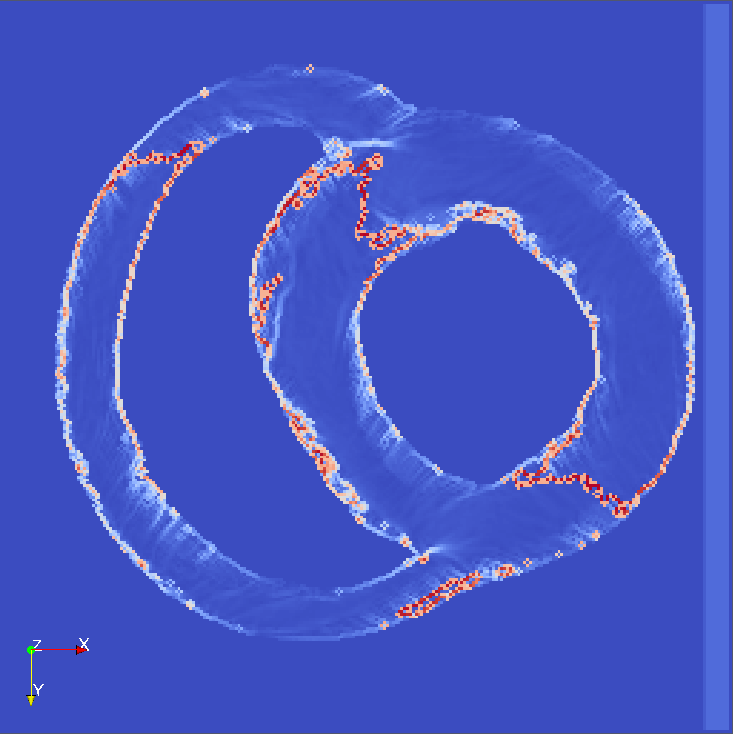
\includegraphics[width=0.9\textwidth]{heart_ftle_org.PNG}
	b)
    \label{b)}
  \end{minipage}
  \begin{minipage}{0.3\textwidth}
  \centering
    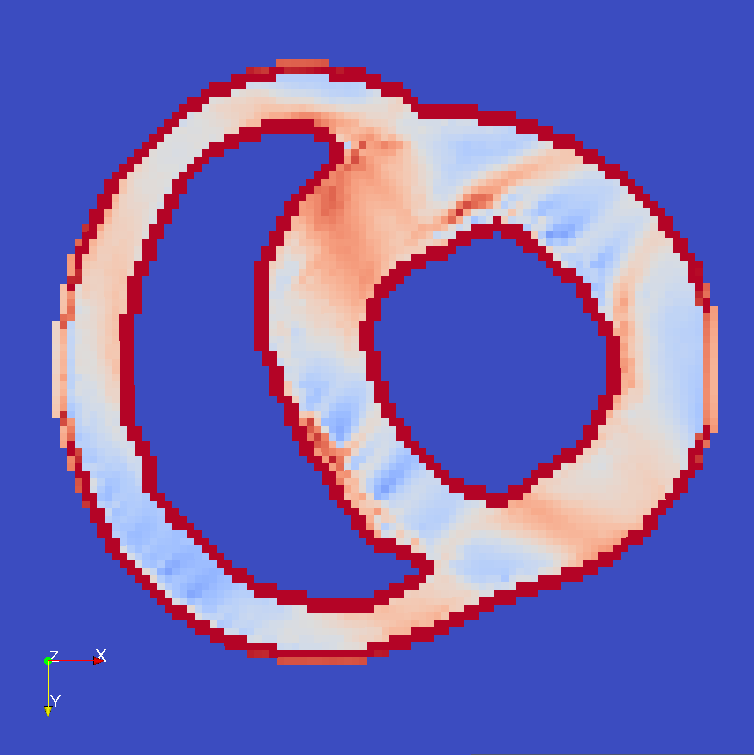
\includegraphics[width=0.9\textwidth]{heart_slice20_rescale.PNG}
	c)
    \label{b)}
  \end{minipage}
  \caption{Heart test field: a) Glyphs, b) LTG local, c) LTG local (rescale)}
\label{heart-ftle}
\end{figure}
\begin{itemize}
	\item light ridges enhanced by rescaling for the down-left direction (red lines in c))
	\item regions exhibit most drastic changes in anisotropy and/or divergence for TFLs
	\item edge artifacts: edges effect high gradients for the flow map
\end{itemize}
} % END OF FRAME


%Volume non-directionally dependent


%%%%%%%%%%%%%%%%%%%%%%%%%%%%%%%%%%%%%%%%%%%%%%%%%%%%%%%%%%%%

% Alternative: put content in separate files
% Check the difference between including these files using \input{filename} and \include{filename} and see which one you like better
%\chapter{Einleitung}\label{intro}
%\input{introduction}
%
%\chapter{Voraussetzungen}\label{bg}
%\input{background}



\end{document}
